% used template from Overleaf: https://www.overleaf.com/latex/templates/academic-paper/rjttmshldvgg

% weird fix for biblatex from: https://tex.stackexchange.com/questions/568021/package-biblatex-error-patching-addtocontents-failed
\let\latexaddtocontents\addtocontents
\documentclass[10pt]{paper}
\let\addtocontents\latexaddtocontents



\usepackage{amssymb}
\usepackage{amsmath}
\usepackage{graphicx}
\usepackage{dcolumn}
\usepackage{hyperref}
\usepackage{float}

\graphicspath{ {./images/} }

\usepackage{biblatex} % https://www.overleaf.com/learn/latex/Bibliography_management_in_LaTeX
\addbibresource{main.bib}

% Code blocks
\usepackage[theme=default]{jlcode}
% \usepackage{listings, xcolor}

% \definecolor{codegreen}{rgb}{0,0.6,0}
% \definecolor{codegray}{rgb}{0.5,0.5,0.5}
% \definecolor{codepurple}{rgb}{0.58,0,0.82}
% \definecolor{backcolour}{rgb}{0.95,0.95,1}

% \lstdefinestyle{mystyle}{
%     backgroundcolor=\color{backcolour},   
%     commentstyle=\color{codegreen},
%     keywordstyle=\color{magenta},
%     numberstyle=\tiny\color{codegray},
%     stringstyle=\color{codepurple},
%     basicstyle=\ttfamily\footnotesize,
%     breakatwhitespace=false,         
%     breaklines=true,                 
%     captionpos=b,                    
%     keepspaces=true,                 
%     numbers=left,                    
%     numbersep=5pt,                  
%     showspaces=false,                
%     showstringspaces=false,
%     showtabs=false,                  
%     tabsize=4
% }

% \lstset{style=mystyle}

\begin{document}

\title{MATH181 Project: Automatic Identification of Nonlinear Systems}
\author{Theo Rode}

% \affiliation{Somewhere}

% \begin{abstract}
% Your abstract.
% \end{abstract}

\maketitle

\section{Introduction} \label{sec:introduction}
Dynamical systems are mathematical objects used to describe anything and everything that changes. This gives rise to their utility in modeling a vast array of real-world systems. Of course, physical systems are of particular interest as the rules of physics work in terms of velocity and acceleration---the descriptors of movement. 
Though, in principle, far more than the cannonical examples of physical movement are ``changing.'' Economic models describe the changes in producer and consumer supply and demand, while biologists model the rise and fall of organism populations in an ecosystem. 
The prevalence of these inherently changing systems leads to the field of dynamical systems having vast applicability to the world of mathematical modeling. Though while they are often the natural language to describe these situations, determining the particular dynamics in a given system is a fundamentally difficult problem. 

This paper discusses a method through which data can be used to uncover the governing equations for a dynamical system. 
%
% This project discusses the procedure of recovering the underlying equations for the dynamics given noisy data collected by the system. So called ``physics-inspired'' or ``physics-informed'' AI.
% The goal of this field is to gain a physical understanding of systems where we can measure various trajectories, but the dynamics are unknown. Though this is additionally useful in situations where complex systems have dynamical properties that can be modeled on a smaller scale. 
In particular, the focus of this paper is on discussing the results demonstrated by Steven Brunton, Joshua Proctor, and Nathan Kutz in their paper published in 2016. They propose a new algorithm for reconstructing dynamics within a system called SINDy (Sparse Identification of Nonlinear Dynamics) \cite{sindy}.
% This first section aims to discuss the field more broadly and relevant papers to the results proposed in the aforementioned paper as well as more generally in the field. 
In this first section, I will discuss the field more broadly prior to Brunton, Proctor, and Kutz publishing their work. This will include a dicussion of relevant papers that provided the groundwork for the SINDy algorithm.
I will then go on to describe relevant mathematical background for SINDy and its underlying mathematics (Section \ref{sec:mathematical_background}). Section \ref{sec:results} will go deeper into the results demonstrated by Brunton et al. by discussing my work to recreate the SINDy algorithm as well as further exploration into the performance of SINDy. 
Finally, section \ref{sec:discussion} offers a dicussion of the results in the paper and further areas of interest. 

The authors of \cite{sindy} give two foundational papers for recovering the dynamics of nonlinear systems: a paper by Josh Bongard and Hod Lipson \cite{bongard} and one by Michael Schmidt and Hod Lipson \cite{schmidt}, in 2007 and 2009 respectively.
Bongard and Lipson \cite{bongard} outline a method for ``reverse engineering'' the dynamics of nonlinear systems by utilizing an active learning system. 
The main process of the algorithm is a technique labeled \textbf{symbolic regression}. Fundamentally, symbolic regression is a regression algorithm that is used to build up arbitrary equations to represent the given data. This is often accomplished through a genetic algorithm where ``function blocks'' are used to build possible functions, which are then tested with the best being used to create the next generation.
In \cite{bongard}, symbolic regression is made usable for complicated (nonlinear) systems by introducing three concepts: partitioning, automated probing, and snipping. Partitioning is a process by which the algorithm is able to model each of the variables in the system separately using stochastic optimization. 
Each of the variables are integrated by substituting in representations of the other variables rather than integrating the variables together. This method significantly reduces the overhead when working with high dimensional systems. Automated probing allows the algorithm to explore the system through active learning. After candidate models are created, the algorithm attempts to create many ``tests'' which are judged against their ability to disprove as many of the candidate models as possible. Then, the test which rejects as many of the candidate models as possible is used to judge the performance of all candidate models in order to pick the most capable ones. From this, the next generation of candidate models can be generated. 
Finally, snipping is a process to reduce the complexity of the generated models and prevent over-fitting. In particular, when creating another generation of models, occasionally certain subexpressions will be replaced with a value of the subexpression picked uniformly from its range. 
This process reduces situations where the model constructs complex subexpressions which take on narrow ranges of values, a hallmark of over-fitting data.
Together, these innovations on the process of symbolic regression allowed Bongard and Lipson to create a framework that was applicable to an array of real-world systems. The framework demonstrated the ability to find nonlinearities and interdependencies as well as an ability to scale successfully. However, the authors note that current limitations include not yet demonstrating scalability to much larger biological models and an inability to work on data where certain variables are unobservable, as a key component of the framework was the active learning \cite{bongard}. 

Schmidt and Lipson present another algorithm for reconstructing dynamics, also based on \textbf{symbolic regression} \cite{schmidt}. 
This paper focuses on presenting a new metric for comparing the accuracy of various candidate equations in order to better search for invariants within the system. 
In particular, once candidate equations are generated (initially randomly from a set of ``building blocks''), the partial derivative pairings of every pair of variables are compared to the numerically calculated 
partial derivative pairings in order to select the equations which model these pairs the closest. They generate the next generation of equations probablistically from the best equations.
To determine the accuracy of equations on the observed data, the authors withhold a random sample from the collected data for testing and when the equations reach a certain level of accuracy, the algorithm terminates.
Finally, equations are prioritized accoriding to measured parsimony---roughly calculated as the number of terms in the expression. 
The authors were able to demonstrate that this algorithm could reconstruct invariants from numerous physical systems effectively. Additionally, they noticed that with a limited set of building blocks, the algorithm found approximations to functions like sines and cosines, utilizing the available building blocks, when such functions were part of the physical invariant \cite{schmidt}. 

% TALK ABOUT MORE RECENT PAPER? 

% mention LASSO: https://watermark.silverchair.com/jrsssb_58_1_267.pdf?token=AQECAHi208BE49Ooan9kkhW_Ercy7Dm3ZL_9Cf3qfKAc485ysgAAA3swggN3BgkqhkiG9w0BBwagggNoMIIDZAIBADCCA10GCSqGSIb3DQEHATAeBglghkgBZQMEAS4wEQQMUUUguuXeXSXLKrHyAgEQgIIDLjjGy45TLem5-SWBsiKqth_ATlBiN1U8oB2jwRawwKAQLhSBq9mr6Xxoy5NWpIW4ICk-qvgW4vlMPUFgp3aXI1CPO7BCP5VER8ruRsVHe-xFxsJrz1Idh0wPazgvEt6cHJfNxeEWOxiBPBYyPMSESASwKHfX4EQxoq_Au2Bzkg6gFRWiGBSestTCekla3yBbmJ9FMWqtL0hVt0LtXXwf81ICM7qX_y4YW0ZKOUS2M9z2EEIMgWCkfeivpJT0CJi8CWfL7oorAsCpsu_wxGucDzNm_Ki_SqlaNZAU-mI3iVIxr4FUCWJxgh8mfeHxCJttaC1p97U5TX3OTzL_S71k4-4DNrWUaGhKgRe2QEXZg8SLWnsRolTN6MBmtlfstqIoMP4PPsaIJ_93YWxRALnL_pdknBTh2edgos_NVDt6nMC41LoCepoI8cSD0BgcJo3L_v3Fa4KOnVHpfLED7PCgj_mT7UY2d4dJlO_3ryWWXa_NhgGbXUywx8KOJzC0M1O0ZAEo0pmz50mMzp0XyVQX6sl3uCHzDB8zHWfI8-BHBzC5dYDHKeGx7xS8H4wws5EriZX_jeHIG4NYUTbCLV0IaVCx4nxTrc6gglm8D2aqlBjI52KHj7iIi78EKZ7pcrgfJ6-RA2rb2435a--KHrXE1S5E4feJA2KWhx7VBEn-t53uszHD7bE3sOrHU7qHDzYKWeuk3T_ewVJuyE8_-P7tLVtWoSKxvsqT1mR4inR6UKmJbHjyTH0HV2QQ6ybtztDj7hrgVPQROkmBMhURkCaGMJHTFeYtdF9W4ZGb7O432f22h7ousNc5dDIAAyGtxGI6doK4bS35eWPzqVMZ5Q4D9WIncF_ehYujzLdosbyNyZLt9SPwaPCBfHwwXCxyDkArH_MWjjOyz-h6D0JxXRyTOyZhw9vbNp8vkpccU0W1zNfmyYn8SkDQJwpN5L1mUpPXeASQb4eH8rE6VttkD09Lmqv4hy502xE-88dYoKVoOToavtAVT9nc-ARwnQ4eyS1dkmPBfy9KOlIz7WHvIg0XFbNoG5AoMjCya6vdfYmDLgNJuhvRVilIhFkuuxMw2cc
% supposedly helpful for sparse regression? 

% talk about advances in compressed sensing seen here: https://journals.aps.org/prl/pdf/10.1103/PhysRevLett.106.154101

\section{Mathematical Background} \label{sec:mathematical_background}
For the SINDy algorithm, the authors aimed to reframe the problem of recovering nonlinear dynamics using \textbf{sparse regression} and \textbf{compressed sensing} \cite{sindy}. Both sparse regression and compressed sensing broadly refer to the process of finding a regression solution to a problem such that the solution is sparse in some function space \cite{sindy}. 
Brunton et al. relate that utilizing sparse regression is a strategy to reduce the noise present in the fitting of systems \cite{sindy}. The particular assumptions for sparse regression come from the idea that in most cases, the dynamics for a particular system will be governed by a small set of given basis functions. Therefore, the sparsity also gives advantages for computation as we can increase the size of the function space dramatically without needing significantly more computation \cite{sindy}. 

% mention LASSO here as alternative method for sparse regression
% The authors of \cite{sindy} propose an iterative algorithm for sparse regression. In particular, they start with a least-squares fit to the data, and then iteratively remove coefficients below a given threshold. By refitting with the remaining, nonzero terms iteratively, the algorithm can arrive at a sparse solution \cite{sindy}. 

The SINDy algorithm relies on the availability of both sampled data, $\mathbf X$, and the sampled derivative, $\mathbf{\dot X}$. However, the authors note that the availability of derivative measurements are not guaranteed and therefore propose using the \textbf{total-variation regularized derivative} to mitigate the noise created from numerically calculating $\mathbf {\dot X}$ from $\mathbf X$ \cite{sindy}. 
In particular, the total-variation regularization technique is attributed to Rudin et al. \cite{rudin}. This method for computing derivatives is robust to noise present in a system, without affect the performance in identifying jump discontinuities \cite{chartrand2011numerical}. 
The implementation of the total-variation regularization derivative is beyond the scope of the paper. 
% Here, Rudin et al. use a framework for computing a desired, denoised output, $u$, from a noisy input, $u_0$, by assuming that $u = u_0 + n$ for some white noise function $n$. It is assumed that $n$ has a mean of $0$ with some given standard deviation. 
% The minmization problem corresponds to minimizing $\int_\Omega \sqrt{u_x^2 + u_y^2} \, \mathrm d A$, which is contrained by $\int_\Omega u \, \mathrm dA = \int_\Omega u_0 \, \mathrm dA$ under the assumption of the additive white noise. It is then proposed to solve for $u$ through either an iterative algorithm (i.e. simulated annealing) or, preferably, a PDE solver to find local minimum \cite{rudin}. 


% In order to address the computational difficulties present in higher-dimensional problems, Brunton et al. suggest using \textbf{proper orthogonal decomposition (POD)} in order to perform dimension reduction \cite{sindy}. 
% Berkooz at el. outline the process of POD on a space of functions \cite{berkooz}. In particular, POD aims to produce a set of vectors (eigenfunctions) and corresponding eigenvalues which best represent a given vector field with coefficients that are uncorrelated (part of a random process) \cite{berkooz}. 
% % https://arc.aiaa.org/doi/epdf/10.2514/1.J058809 (POD)

\subsection{SINDy} \label{sec:SINDy}
The main purpose of SINDy is in identifying the function $\mathbf f$ in (\ref{eq:dynamical_system}). 
\begin{equation}\label{eq:dynamical_system}
	\frac{\mathrm d}{\mathrm dt} \mathbf x(t) = \mathbf f (\mathbf x(t)).
\end{equation}
Such identification requires the collection of timeseries data, $\mathbf X$. The form of $\mathbf X$ is as follows: 

% In order to use the concepts of sparse regression and compressed sensing, discussed above, the authors assume that $\mathbf f$ is sparse in some function space \cite{sindy}.
% The state vector, $\mathbf x(t)$, is collected over some time period and $\mathbf {\dot x}$ is either sampled alongside $\mathbf x(t)$ or numerically calculated from it. 
% These samplings create the following matrices: 
\[ \mathbf X = \begin{bmatrix}
	\mathbf x^T(t_1) \\ \mathbf x^T(t_2) \\ \vdots \\ \mathbf x^T(t_m)
\end{bmatrix} = \begin{bmatrix}
	x_1(t_1) & x_2(t_1) & \cdots & x_n(t_1) \\
	x_1(t_2) & x_2(t_2) & \cdots & x_n(t_2) \\
	\vdots & \vdots & \ddots & \vdots \\ 
	x_1(t_m) & x_2(t_m) & \cdots & x_n(t_m)
\end{bmatrix}, \]  
where each row of $\mathbf X$ is some measurement in time of the $n$ state variables in our system. Hence, the columns of $\mathbf X$ correspond to the different state variables of our system, and the rows of $\mathbf X$ represent timeseries data measurements from our system. Either sampled alongside $\mathbf X$, or numerically computed from it, we also need the relevant derivatives, 
\[ \mathbf {\dot X} = \begin{bmatrix}
	\mathbf {\dot x}^T(t_1) \\ \mathbf {\dot x}^T(t_2) \\ \vdots \\ \mathbf {\dot x}^T(t_m)
\end{bmatrix} = \begin{bmatrix}
	\dot x_1(t_1) & \dot x_2(t_1) & \cdots & \dot x_n(t_1) \\
	\dot x_1(t_2) & \dot x_2(t_2) & \cdots & \dot x_n(t_2) \\
	\vdots & \vdots & \ddots & \vdots \\ 
	\dot x_1(t_m) & \dot x_2(t_m) & \cdots & \dot x_n(t_m)
\end{bmatrix}. \]  
As discussed above, Brunton et al. propose using the total-variation regularization derivative to combat noise if numerically calculating $\mathbf {\dot X}$ from $\mathbf X$. 
It is important to note that no assumptions are made about the time steps between each $t_i$, nor do all collected data points need to be from the same orbit. 

In order to specify the particular function basis we aim to use for SINDy, we construct a function library. In essence, this library is constructed such that each column is representative of a candidate function in our function basis, 
\[ \Theta(\mathbf X) = \begin{bmatrix}
	g_1(\mathbf x(t_1)) & g_2(\mathbf x(t_1)) & \cdots & g_k(\mathbf x(t_1)) \\ 
	g_1(\mathbf x(t_2)) & g_2(\mathbf x(t_2)) & \cdots & g_k(\mathbf x(t_2)) \\ 
	\vdots & \vdots & \ddots & \vdots \\ 
	g_1(\mathbf x(t_m)) & g_2(\mathbf x(t_m)) & \cdots & g_k(\mathbf x(t_m)) 
\end{bmatrix}. \]
In principle, each $g_i$ could be any function in terms of any subset of the state variables. Computation of $\Theta(\mathbf X)$ simply amounts to the evaluation of these candidate functions on all timeseries measurements from our system. 
We will seek a solution for the governing equation of each state variable as some linear combination of these candidate functions, 
\[ \dot x_i(t) = \xi_{i, 1}g_1(\mathbf x(t)) + \xi_{i, 2}g_2(\mathbf x(t)) + \cdots + \xi_{i, k}g_k(\mathbf x(t)). \]
In particular, we seek a sparse solution, meaning that most of the coefficients are zero (most $\xi_{i, j} = 0$). 
In practice, our function library could contain a mixture of polynomial terms and sines or cosines, 

\[  \Theta(\mathbf X) = \begin{bmatrix} \mid & \mid & \mid & \mid &  & \mid & \mid & \\ 1 & \mathbf X & {\mathbf X}^{P_2} & {\mathbf X}^{P_3} & \cdots & \sin{(\mathbf X)} & \cos{(\mathbf X)} & \cdots \\ \mid & \mid & \mid & \mid & & \mid & \mid & \end{bmatrix}.  \]
Here, $\mathbf X^{P_2}$ represents the quadratic nonlinearities in $\mathbf f$, 
\[ \mathbf X^{P_2} = \begin{bmatrix}
	x_1^2(t_1) & x_1(t_1)x_2(t_1) & \cdots & x_1(t_1)x_n(t_1) & x_2^2(t_1) & \cdots & x_n^2(t_1) \\
	x_1^2(t_2) & x_1(t_2)x_2(t_2) & \cdots & x_1(t_2)x_n(t_2) & x_2^2(t_2) & \cdots & x_n^2(t_2) \\
	\vdots & \vdots & \ddots & \vdots & \vdots & \ddots & \vdots \\
	x_1^2(t_m) & x_1(t_m)x_2(t_m) & \cdots & x_1(t_m)x_n(t_m) & x_2^2(t_m) & \cdots & x_n^2(t_m) \\
\end{bmatrix}, \]
while $\sin{(\mathbf X)}$ would be 
\[ \sin{(\mathbf X)} = \begin{bmatrix}
	\sin(x_1(t_1)) & \sin(x_2(t_1)) & \cdots & \sin(x_n(t_1)) \\ 
	\sin(x_1(t_2)) & \sin(x_2(t_2)) & \cdots & \sin(x_n(t_2)) \\
	\vdots & \vdots & \ddots & \vdots \\ 
	\sin(x_1(t_m)) & \sin(x_2(t_m)) & \cdots & \sin(x_n(t_m))
\end{bmatrix}. \]
After constructing our function library, we may continue by solving the sparse regression problem, 
\[ \mathbf {\dot X} = \Theta(\mathbf X)\mathbf \Xi. \]
In particular, we aim to find a $\mathbf \Xi$, similar to a traditional least-squares regression, such that $\mathbf \Xi$ is sparse. 
A further discussion of the mechanisms for performing this sparse regression are discussed in Section \ref{sec:code}. 
We note that $\mathbf \Xi = \begin{bmatrix}
	\boldsymbol \xi_1 & \boldsymbol \xi_2 & \cdots & \boldsymbol \xi_n
\end{bmatrix}$ where each $\boldsymbol \xi_i$ is a sparse vector dictating the coefficients on the candidate functions for the governing equation of state variable $x_i$. 

The authors additionally suggest an alteration to the algorithm in order to detect bifurcations present in a system. In particular, the authors appended the bifurcation parameter to the dynamics: 
\begin{equation} \label{eq:sindy_with_bifurcation}
	\begin{split}
		\mathbf {\dot x} &=  \mathbf{f}(\mathbf x; \mu), \\
		\dot \mu &= 0.
	\end{split}
\end{equation}
Then, by sampling data from different values of $\mu$, it is possible for SINDy to reconstruct the system from combinations of $\mathbf x$ as well as $\mu$. 
This results in an identified system that can capture the bifurcation behavior in changes of $\mu$. 

\section{Results} \label{sec:results}
\subsection{Code} \label{sec:code}
Central to recreating the results presented by Brunton et al. was writing a novel implementation of the SINDy algorithm.
I wrote the code in the Julia Programming Language \cite{julia}.
All data used to train the SINDy model was collected by integrating using ordinary differential equation (ODE) solvers provided by the DifferentialEquations.jl \cite{rackauckas2017differentialequations} package.

In order to replicate sensor noise, randomly sampled noise from a standard normal distribution was added to all collected data ($\mathbf X$).
This noise was scaled by some noise mangitude, $\eta$, in order to test the performance of SINDy at various levels of system noise. Additionally, all derivatives $(\mathbf {\dot X}$) were numerically calculated from the data after noise was applied. 
Distributions.jl \cite{JSSv098i16}\cite{Distributions.jl-2019} was used to sample the noise and NoiseRobustDifferentiation.jl \cite{chartrand2011numerical}\cite{NoiseRobustDifferentiation.jl} provided an implementation of the total-variation regularization derivative in order to compute $\mathbf{\dot X}$. 

Utilizing the data matrix, $\mathbf X$, it is then simple to construct the function library, $\mathbf \Theta(\mathbf X)$.
Unlike the original paper \cite{sindy}, this implementation allows for arbitrary functions to be used and provides a framework for easily expanding the type and quantity of functions used. 
In particular, along with the potential to fit arbitrary functions, the generation of polynomial terms was done generally to support arbitrary degree polynomials utilizing functions Combinatorics.jl \cite{Combinatorics.jl}.

Finally, the sparse regression algorithm to compute $\mathbf \Xi$ is the same process as outlined by Brunton et al. \cite{sindy}. The code for this algorithm is shown in Listing \ref{lst:sparse_regression}.
In particular, the algorithm starts by taking an initial ordinary least squares solution for $\mathbf \Xi$. Following this, the algorithm iteratively finds and removes coefficients in $\mathbf \Xi$ under some sparsity parameter, $\lambda$. On each iteration, after finding these small coefficients, we set these coefficients to zero and re-regress on only the remaining non-zero terms. 
Brunton et al. found that this algorithm converges rapidly (for a few iteration steps), meaning that 5-10 iterations are often sufficient. 

% \jlinputlisting[language = Julia, caption = {Sparse regression}, label = {sparse_regression}, firstline = 3, lastline = 23, float, floatplacement = ptb]{../Code/DynamicsRecovery/src/SINDy/sparse_regression.jl}
\begin{jllisting}[language = Julia, caption = {Sparse regression}, label = {lst:sparse_regression}, float, floatplacement = ptb]
function sparse_regression(Θ::Matrix{Float64}, Xdot::Matrix{Float64}, λ::Float64, kmax::Integer) 
    # create initial guess for Xi as just regression
    Ξ = Θ\Xdot

    for _ in 1:kmax 
        # find coefficients that are less than λ 
        small_coefficients = abs.(Ξ) .< λ

        # set small coefficients to 0 
        Ξ[small_coefficients] .= 0

        # now individually run regression on non-zero coefficients
        for n in 1:(size(Xdot)[2]) # loop through all state dimensions 
            nonsmall = .!small_coefficients[:, n]
            
            Ξ[nonsmall, n] = Θ[:, nonsmall]\Xdot[:, n]
        end # for n
    end # for k 

    Ξ
end # function sparse_regression
\end{jllisting}
After this process, $\mathbf \Xi$ defines a ``discovered system'' from the data. In particular, we can use this discovered system to project dynamics for the original system. 

% The resulting system defined by $\mathbf \Xi$ can then be solved using the same methods as when collecting data for the original system. The governing equations are constructed using the same function generation from the library construction in order to ensure complete generality. 

\subsection{Measuring Error} \label{sec:measuring_error}
In order to discuss the performance of SINDy, I aim to propose an error metric that accounts for the overall scale of the system, as well as a desire to improve the accuracy of the derivative over that of the orbit. A particular case study for the importance of emphasizing derivative accuracy over orbit accuracy is that of a chaotic system, where it would be reasonable to expect large deviations in orbits with derived systems closely matching the actual, underlying system. 
Therefore, qualitatively similar behavior could be labeled as inaccurate due to expected deviations from small variations in parameters. Further, we want an error metric to be proportional to the overall scale of the system, as scaling the coordinate system shouldn't change the accuracy of the derived system. 
For fulfilling these requirements, the following error metric may be used: 
\[ \varepsilon = \sqrt{ \left( \sum_{i \in T} \frac{(\dot x_1(t_i) - f_1(t_i))^2}{\sum_{i \in T} (\dot x_1(t_i))^2} \right)^2 + \cdots + \left( \sum_{i \in T} \frac{(\dot x_n(t_i) - f_n(t_i))^2}{\sum_{i \in T} (\dot x_n(t_i))^2} \right)^2 }, \]
where $T$ is a set of indices for the collected timeseries data, $\dot x_j(t_i)$ is the measured derivative from the system for state variable $j$ and time $i$, $f_j(t_i)$ is the same but for the found sytem, and $n$ is the state dimension. 
Typically, cross-validation techniques are used to test the accuracy of a fit, where a certain proportion of the collected data is withheld in order to calculate this error. Hence, $T$ represents that subset of data withheld for testing. 
In particular, this error metric can be thought of as how large, in proportion to the magnitude of the derivative of the system, the error in the derivative is for the found system. Throughout this paper I will cite this error metric for found systems to give an idea of the relative performance of SINDy between cases. 
As a standard, error will be calculated on 10 percent of the data randomly selected to be withheld for testing. 

\subsection{The Lorenz Attractor} \label{sec:lorenz_results}
In replicating the results of Brunton et al., I first pursued replicating the success they found in recoverying the dynamics present in the chaotic Lorenz System \cite{sindy}\cite{lorenz1963deterministic}. 
The dynamics for this system are governed by the following equations, 
\begin{equation}\label{eq:lorenz}
\begin{split}
	\dot x &= \sigma(y - x), \\
	\dot y &= x(\rho - z) - y, \\
	\dot z &= xy - \beta z.
\end{split}
\end{equation}
I used the same initial conditions and parameters that Brunton et al. \cite{sindy} used for their demonstrations. In particular, $u_0 = (-8, 7, 27)$ and parameters $(\sigma, \rho, \beta) = \left( 10, 28, \frac 83 \right)$. 
Figure \ref{fig:lorenz_system_actual} shows the actual system with these parameters and initial condition. 

\begin{figure}[h]
	\caption{Lorenz system}
	\label{fig:lorenz_system_actual}

	\centering
	\includegraphics[width = 0.47\textwidth, trim={4.3cm, 1.6cm, 4.3cm, 2.5cm}, clip]{lorenz_attractor.pdf}
\end{figure}

In this section, I will examine the performance of the SINDy algorithm across different magnitudes of noise applied to sampled points from the system. 
In particular, I will demonstrate results for noise magnitudes $\eta = 0.01$, $\eta = 0.1$, and $\eta = 1$ where noise is generated by sampling from a standard normal distribution, and scaling the sampled noise by $\eta$. 
Further, it is important to note that noise is applied to the data matrix, $\mathbf X$, before the derivatives, $\mathbf {\dot X}$ is computed. 
The derivatives are computed numerically from the sampled data after noise application, so in order to counteract the noise in the data, derivatives are calculated using the total-variation regularization derivative, as suggested by Brunton et al. \cite{sindy}. 
Data was collected with a timespan from $0$ to $100$, with $dt = 0.001$. For measuring error, $10\%$ of the collected data was withheld as testing data to compare against. 
The results for the different levels of noise can be seen in Figure \ref{fig:found_lorenz_systems}.
\begin{figure}[h]
	\caption{Discovered Lorenz systems with noise magnitudes $\eta = 0.01$, $\eta = 0.1$, and $\eta = 1$. Error ($\varepsilon$) is reported as described in Section \ref{sec:measuring_error}.}
	\label{fig:found_lorenz_systems}

	\centering 
	\begin{minipage}{0.32\textwidth}
		\[ \eta = 0.01, \, \lambda = 0.25, \]
		\[ \varepsilon = 0.00041 \]
		\begin{center}
			\includegraphics[width = 0.95\textwidth, trim={4.3cm, 1.6cm, 4.3cm, 2.5cm}, clip]{found_lorenz_001.pdf}
		\end{center}
		\resizebox{!}{1.75em}{$\begin{aligned} 
			\dot x &=-9.945x + 9.975y \\ 
			\dot y &= 27.063x  -0.674y  -0.977xz\\ 
			\dot z &= -2.649z + 0.996xy
		\end{aligned}$}
	\end{minipage}%
	\begin{minipage}{0.32\textwidth}
		\[ \eta = 0.1, \, \lambda = 0.4, \]
		\[ \varepsilon = 0.00301 \]
		\begin{center}
			\includegraphics[width = 0.95\textwidth, trim={4.3cm, 1.6cm, 4.3cm, 2.5cm}, clip]{found_lorenz_01.pdf}
		\end{center}
		\resizebox{!}{1.75em}{$\begin{aligned} 
			\dot x &= -9.800x + 9.832y \\ 
			\dot y &= 25.948x  -0.438y -0.947xz \\ 
			\dot z &= -2.615z + 0.983xy
		\end{aligned} $}
	\end{minipage}%
	\begin{minipage}{0.32\textwidth}
		\[ \eta = 1, \, \lambda = 0.416, \]
		\[ \varepsilon = 0.21021 \]
		\begin{center}
			\includegraphics[width = 0.95\textwidth, trim={4.3cm, 1.6cm, 4.3cm, 2.5cm}, clip]{found_lorenz_1.pdf}
		\end{center}
		\resizebox{!}{1.75em}{$\begin{aligned} 
			\dot x &= -7.007x + 7.148y  \\ 
			\dot y &= 14.836x + 1.578y  -0.631xz \\ 
			\dot z &=   -2.149z + 0.839xy -2.150
		\end{aligned}$}
	\end{minipage}
\end{figure}	


We can see that for the three noise levels, SINDy was able to correctly identify the qualitative behavior of the Lorenz system. 
Further, SINDy identifies exclusively the correct terms in the systems for $\eta = 0.01$ and $\eta = 0.1$, deviating from the expected terms in $\eta = 1$ by a forcing term in the $\dot z$ equation (Figure \ref{fig:found_lorenz_systems}). 
Additionally, we notice that error in the produced system increases with noise, as we may expect, but additionally that this increase in error is not linear with noise. In particular, while the $\eta = 0.1$ system has approximately 10-fold the error as the $\eta = 0.01$ system, the $\eta = 1$ system sees an 100-fold increase in error over $\eta = 0.1$.   

For completeness, we note that for the $\eta = 0.01$ system, we use the basis $$\mathcal B = \{ \mathbf 1, \mathbf X, \mathbf X^{P_2}, \ldots, \mathbf X^{P_7}, \sin(1\mathbf X), \ldots, \sin{10\mathbf X}, \cos{1\mathbf X}, \ldots, \cos{10\mathbf X} \}.$$ We use a smaller basis for $\eta = 0.1$, $$\mathcal B = \{  \mathbf 1, \mathbf X, \mathbf X^{P_2}, \ldots, \mathbf X^{P_5}, \sin(1\mathbf X), \ldots, \sin{10\mathbf X}, \cos{1\mathbf X}, \ldots, \cos{10\mathbf X}\},$$ 
and a smaller basis still for $\eta = 1$, 
\[ \mathcal B = \{ \mathbf 1, \mathbf X, \mathbf X^{P_2}, \ldots, \mathbf X^{P_5} \}. \]
The choice of basis was motivated by accuracy concerns with the higher levels of noise. For a larger discussion of the basis choice, see Appendix \ref{apx:lorenz_with_diff_bases}.

\subsection{Bifurcations: The Hopf normal form} \label{sec:hopf_results}
In addition to SINDy's ability to recover the qualitatively similar dynamics to the chaotic Lorenz attractor, simple modifications to the SINDy algorithm, as discussed in Section \ref{sec:SINDy}, can allow SINDy to find bifurcations present in a system. 
As a case study on this ability, I will investigate the Hopf normal form and SINDy's ability to reconstruct the Hopf bifurcation present in the system. The Hopf normal form is given by the governing equations in (\ref{eq:hopf_normal}).
\begin{equation} \label{eq:hopf_normal}
	\begin{split}
		\dot x &= \mu x - \omega y - Ax(x^2 + y^2), \\
		\dot y &= \omega x +\mu y - Ay(x^2 + y^2).
	\end{split}
\end{equation} 
In this section, I take parameter values $\omega = A = 1$, and collect data over a range of values for $\mu$, the bifurcation parameter (note the bifurcation occurs when $\mu$ goes from negative to positive). 
A bifurcation diagram of the Hopf normal form can be seen in Figure \ref{fig:hopf_normal_form}. 
\begin{figure}[h]
	\caption{Bifurcation diagram for the Hopf normal form. Blue orbits have initial condition $(x_0, y_0) = (2,0)$ and red orbits have initial condition $(x_0, y_0) = (0.01, 0)$. 
	$\mu$ takes on values $\mu \in \{-0.2, -0.15, -0.1, -0.05, 0, 0.05, 0.1, 0.15, 0.2 \}$.}
	\label{fig:hopf_normal_form}
	\centering 

	\includegraphics[width = 0.7\textwidth, trim={4.3cm, 2cm, 4.2cm, 3cm}, clip]{hopf_normal_actual.pdf}

\end{figure}
For sampling data from the system, I sampled from 17 values of $\mu$ between $\mu = -0.3$ and $\mu = 0.55$, where for negative values of $\mu$ I took one initial condition in a neighborhood of $(x_0, y_0) = (2, 0)$, while for positive values of $\mu$ I took one orbit form an initial condition in that neighborhood, and one from a neighborhood around $(x_0, y_0) = (0.01,0)$. In particular, the initial conditions were picked by some random perturbation from $(2,0)$ and $(0.01, 0)$ in order to achieve more diversity in the data. 
Finally, noise with magnitude $\eta = 0.005$ was applied to all collected data and $10\%$ of the data was withheld for error reporting.  
All derivatives were computed using the total-variation regularization derivative to reduce the effect of noise. A basis of all $5$th-degree polynomials was used with sparsity parameter $\lambda = 0.6$. The resulting system is shown in Figure \ref{fig:discovered_hopf_0005}.

\begin{figure}[h]
	\caption{Discovered Hopf bifurcation with noise $\eta = 0.005$. Blue orbits have initial condition $(x_0, y_0) = (2,0)$ and red orbits have initial condition $(x_0, y_0) = (0.01, 0)$. Error, calculated as described in Section \ref{sec:measuring_error}, is $\varepsilon = 0.00913$.}
	\label{fig:discovered_hopf_0005}

	\centering 

	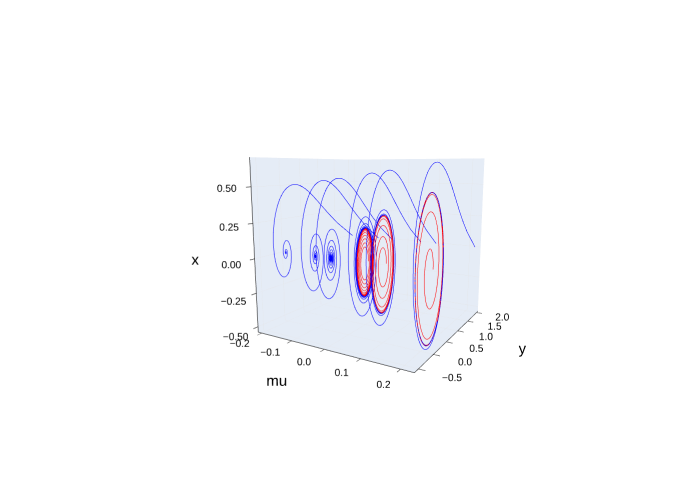
\includegraphics[width = 0.7\textwidth, trim={4.3cm, 2cm, 4.2cm, 3cm}, clip]{found_hopf_bifurcation_0005.pdf}

	\[ \begin{aligned}
		\dot x &= -0.972y + 0.952x\mu -0.919x^3 -1.025xy^2 \\
		\dot y &= 0.952x + 0.959y\mu -0.946y x^2 -0.956y^3 + 0.629\mu x y^2 -0.624xy^2\mu^2
	\end{aligned} \]

\end{figure}

Of particular interest, SINDy was able to correctly identify the qualitative behavior of the Hopf normal form, and the bifurcation occuring at $\mu = 0$. Additionally, it identified the correct basis terms for the $\dot x$ equation exactly, while for the $\dot y$ term it included an extra $\mu xy^2$ and $xy^2\mu^2$ terms. 
Additionally, the error measured in this system is higher than the noise observed in the Lorenz system for $\eta = 0.01$ and $\eta = 0.1$, both representing a larger magnitude of noise. This is indicative of different performance characteristics for SINDy depending on the system in question. We see this effect further with the Hopf normal form, as while the discovered Lorenz systems were similar with run-to-run noise variability, the Hopf normal form could have variable results with a different noise sample. 
In particular, we can see this in Figure \ref{fig:discovered_hopf_0005_2} where a different noise sample increases the error by about 3-fold, and changes the erronous terms identified by SINDy. 

\begin{figure}[H]
	\caption{Discovered Hopf bifurcation with noise $\eta = 0.005$ (but different noise sample from Figure \ref{fig:discovered_hopf_0005}). Blue orbits have initial condition $(x_0, y_0) = (2,0)$ and red orbits have initial condition $(x_0, y_0) = (0.01, 0)$. Error, calculated as described in Section \ref{sec:measuring_error}, is $\varepsilon = 0.02902$.}
	\label{fig:discovered_hopf_0005_2}

	\centering 

	\includegraphics[width = 0.7\textwidth, trim={4.3cm, 2cm, 4.2cm, 3cm}, clip]{found_hopf_bifurcation_0005_2.pdf}

	\[ \begin{aligned}
		\dot x &= -0.971y + 0.940\mu x -0.911x^3 -1.148xy^2 + 0.674xy^2\mu^2 \\
		\dot y &= 0.966x + 0.955\mu y -0.924x^2 y -0.955y^3
	\end{aligned} \]

\end{figure}

\subsection{Determining the Sparsity Parameter} \label{sec:determining_lambda}
Brunton et al. discuss the concept of picking the sparsity parameter, $\lambda$, on the ``Pareto front'' where we see a balancing of complexity and accuracy \cite{sindy}. 
Such an approach involves picking $\lambda$ when we see a sharp increase in accuracy when increasing the complexity of the model. 
We can see this jump in accuracy behavior in Figure \ref{fig:large_scale_sparsity_error}, where we see accuracy dramatically rise (an increase in the negative error) at a particular sparsity. 

\begin{figure}[H]
	\caption{Measured sparsity (percent non-zero coefficients) graphed against the negative error ($\varepsilon$) as discussed in Section \ref{sec:measuring_error}. Parameterized by $\lambda$ between $14.98$ and $0$.}
	\label{fig:large_scale_sparsity_error}
	\centering 

	\includegraphics[width = 0.7\textwidth]{large_scale_error_sparsity.pdf}
\end{figure}
We additionally see another (proportionally similar in size) jump following the initial jump in accuracy (Figure \ref{fig:small_scale_sparsity_error}).
\begin{figure}[h]
	\caption{Measured sparsity (percent non-zero coefficients) graphed against the negative error ($\varepsilon$) as discussed in Section \ref{sec:measuring_error}. Parameterized by $\lambda$ between $0.943$ and $0$.}
	\label{fig:small_scale_sparsity_error}
	\centering 

	\includegraphics[width=0.7\textwidth]{small_scale_error_sparsity.pdf}

\end{figure}
The jumps in error occur at $\lambda = 0.9434$, $\lambda = 0.674$, $\lambda = 0.0599$, and $\lambda = 0.0300$. We can examine the performance of SINDy with each of these sparsity parameters (Figure \ref{fig:lambda_variation}) and see that in each case, a decrease in $\lambda$ corresponds to an additional term added in the found system. 
Indeed, the initial jump from $\lambda = 0.9434$ to $\lambda = 0.6739$ sees a jump to the identification of only the correct terms, while smaller values of $\lambda$ introduce extra terms evident of over-fitting. 


\begin{figure}[ptb]
	\caption{Discovered Lorenz Systems with noise $\eta = 0.01$ across different sparsity parameters ($\lambda$) specific to jumps in error ($\varepsilon$).}
	\label{fig:lambda_variation}
	\centering 

	\begin{minipage}{0.47\textwidth}
		\[ \lambda = 0.9434, \, \varepsilon = 0.00125 \] 
		\begin{center}
			\includegraphics[width=0.95\textwidth, trim={4.3cm, 1.6cm, 4.3cm, 2.5cm}, clip]{lorenz_lambda_1.pdf}
		\end{center}
		\[ \begin{aligned}
			\dot x &= -9.945x + 9.975y \\
			\dot y &= 25.393x -0.944xz\\ 
			\dot z &= -2.649z + 0.996xy \\ 
		\end{aligned} \]

		\vspace{1em}

		\[ \lambda = 0.0599, \, \varepsilon = 0.00038 \]
		\begin{center}
			\includegraphics[width=0.95\textwidth, trim={4.3cm, 1.6cm, 4.3cm, 2.5cm}, clip]{lorenz_lambda_3.pdf}
		\end{center}
		\[ \begin{aligned}
			\dot x &= -9.945x + 9.975y \\ 
			\dot y &= 27.0627x -0.674y  -0.977xz \\ 
			\dot z &=  -2.578z + 0.996xy -1.910
		\end{aligned} \]
	\end{minipage}%
	\begin{minipage}{0.47\textwidth}
		\[ \lambda = 0.6739, \, \varepsilon = 0.00041 \]
		\begin{center}
			\includegraphics[width=0.95\textwidth, trim={4.3cm, 1.6cm, 4.3cm, 2.5cm}, clip]{lorenz_lambda_2.pdf}
		\end{center}
		\[ \begin{aligned}
			\dot x &= -9.945x + 9.975y \\ 
			\dot y &= 27.063x -0.674y  -0.977xz\\ 
			\dot z &= -2.649z + 0.996xy\\ 
		\end{aligned} \]

		\vspace{1em}

		\[ \lambda = 0.0300, \, \varepsilon = 0.00035 \]
		\begin{center}
			\includegraphics[width=0.95\textwidth, trim={4.3cm, 1.6cm, 4.3cm, 2.5cm}, clip]{lorenz_lambda_4.pdf}
		\end{center}
		\[ \begin{aligned}
			\dot x &=-9.945x + 9.975y \\ 
			\dot y &= 27.0627x -0.674y -0.977xz \\ 
			\dot z &= 0.579 -2.720z + 0.038x^2 + 0.972xy
		\end{aligned} \] 
	\end{minipage}
\end{figure}

It is important to recognize that decreasing $\lambda$, in this case, is always leading to a decrease in error, $\varepsilon$. However, as we see the slow introduction of forcing terms, such a decrease in $\lambda$ can result in symptoms of over-fitting. Therefore, any automated finding of a sparsity parameter needs to consider the potential for such over-fitting, and adjust accordingly. 

From this, we may propose a simple algorithm for finding an ideal $\lambda$ for a given system. In particular, we start from $\lambda = 0$ and increase $\lambda$ by repeatedly choosing $\lambda$ to be the smallest element (plus some small constant) of our fit $\mathbf \Xi$.
This allows us to quickly cycle through values of $\lambda$ that are guaranteed to change the fit. We look for a change in $\lambda$ that corresponds to a relatively large jump in error, $\varepsilon$. 
When we observe this jump, we can more precisely search the space between the two values of $\lambda$ where the jump occured to get the largest value of $\lambda$ that lies before the jump in error. 
By doing this, we can search for an ideal value for $\lambda$ that attempts to avoid over-fitting. Effectively searching the space for the ``Pareto front'' desrcibed by Brunton et al. \cite{sindy}. 

By running this algorithm on the Lorenz systems described in Section \ref{sec:lorenz_results}, we find that it produces the same systems as shown in Figure \ref{fig:found_lorenz_systems}, though with $\lambda = 0.620024$, $\lambda = 0.920751$, and $\lambda = 0.414742$, respectively. 
These values for $\lambda$ are significantly larger (or very similar) to those used in \ref{sec:lorenz_results}, demonstrating that there is significant headroom in choosing values for $\lambda$. Additionally, with these values of $\lambda$ determined entirely algorithmically, whereas $\lambda$ values were chosen by hand in Section \ref{sec:lorenz_results}, we demonstrate suitability of this sparsity parameter finding algorithm. 




\section{Discussion} \label{sec:discussion}

In writing a ground-up implementation of the SINDy algorithm, I was able to replicate much of the success found by Brunton et al. in their paper presenting SINDy \cite{sindy}. 
In particular, I was able to demonstrate remarkable success in replicating the qualitative behavior of both chaotic systems (Figure \ref{fig:found_lorenz_systems}) as well as systems with bifurcations (Figure \ref{fig:discovered_hopf_0005} and Figure \ref{fig:discovered_hopf_0005_2}).
Further, these examples demonstrated an ability for SINDy to correctly determine the function basis elements present in the governing equations for these systems. 
In all, this demonstrates a remarkable ability for SINDy to be used to gleam insights into the underlying dynamics of a system when only time series data on the system is available. 

However, it is important to note that I observed run to run variability in the success of the SINDy algorithm as discussed in Section \ref{sec:hopf_results}.
This demonstrates that SINDy can be particularly sensitive to noise depending on the system in question. Of particular concern is the potential increase in error from simply differently sampled noise (the example presented in this paper showed a 3-fold increase in error). This is additionally interesting as such variability in results was not found for the Lorenz system (Section \ref{sec:lorenz_results}). 

Another condition on the performance of the SINDy algorithm is the choice of basis. Brunton et al. emphasize the necessity of a properly chosen basis in their work \cite{sindy}, and I was also able to demonstrate this sensitivity to the basis chosen. 
A deeper discussion on the instability noticed for different bases when running SINDy on the Lorenz System is noted in Appendix \ref{apx:lorenz_with_diff_bases}, however as summary, the choice of basis is not simply in exhaustion of potential function candidates, but can also cause SINDy to perform worse if the solution is too sparse in the chosen basis. 
Further, SINDy can show instability with single function additions to the basis, and fails to perform at all when the basis doesn't contain the necessary function candidates. 

For these reasons, exploring methods to determine good bases for SINDy is a fruitful area of further exploration.
If such methods could increase the stability of SINDy, they could dramatically improve its usability. Without trust in the solutions produced, particularly with possible variations simply down to noise, it would be difficult to deploy SINDy to an application where the derived system would need to be trusted. 
A possible extention to address these issues could also be in the form of active learning with the SINDy algorithm. Fasel et al. propose a modification to SINDy with control in order to implement said active learning into SINDy \cite{9683120}. 
Further, more investigations into the performance of SINDy in situations where the governing equations are not known would be useful, in order to determine the usefulness of SINDy when parameters have to be determined without a reference to the actual, underlying system. 

Despite the difficulties in the consistency of SINDy, the applications for such a system could be expansive. In systems where non-conventional dynamical systems may apply, an algorithm like SINDy could be used to create a guess at the underlying dynamics in order to improve projections. 
A situation such as the stock market may be an interesting area of study using SINDy, or a similar algorithm, as the dynamics of the stock market are heavily obfuscated and potentially such an algorithm could gleam useful information on the dynamics from just the data. 
Robotic applications such as surface finishing could also potentially benefit from an algorithm such as SINDy. 
In particular, the response to pressure from the end-effector on a part could have implications on the quality of the ultimate finishing job. 
If imperfect, but generally accurate systems could be constructed to model such feedback, it could greatly improve the robot's understanding of the part and how to finish it. 

In an effort to explore further systems where SINDy could be applied, I worked to use SINDy to recover the dynamics from a three-body gravitational system (three-body problem). This is another cannonical example of a chaotic system (like the Lorenz system). 
However, I was unable to find success with SINDy in this system, with the lowest error achieved being $\varepsilon = 14.755$. Part of the problem with applying SINDy to this particular system is the scale and frequency of extreme behavior present in the three-body system. 
This erratic behavior likely creates a difficult environment for SINDy to operate. Additionally, SINDy could be struggling due to this being the only system tested that does not use a strictly polynomial basis. In particular, this system has the cube of a vector norm in the demoninator of the governing equations, necessitating a much more complicated function basis then either the Lorenz system or the Hopf normal form. 
While I was unable to achieve success in this system, further exploration on the prospects of modeling the three-body problem with SINDy are likely required. Additionally, further investigation of modeling other systems could bring to light additional drawbacks with the SINDy algorithm. 

While the SINDy algorithm shows immense promise in its ability to identify these systems, questions of stability and ability to choose a proper basis remain. These concerns make SINDy more difficult to apply in real-world scenarios, where the actual underlying system is unknown. 
In these situations, it becomes less clear if the system SINDy finds is reasonable, and therefore whether or not a different basis (or parameter values) should be used.
Though these concerns remain, SINDy is significantly more powerful than the algorithms that inspired it \cite{bongard}\cite{schmidt}. This trajectory suggests a promising future for dynamics recovery algorithms.  


% \section{}
% \label{sec:examples}

% \subsection{Sections}




% \begin{acknowledgments}

% We thank\dots

% \end{acknowledgments}

\appendix 
\newpage 
\section{Lorenz System with Different Bases} \label{apx:lorenz_with_diff_bases}
It is important to illustrate the sensitivity of the SINDy algorithm on the chosen basis. For the Lorenz System, performance was strong for bases that included a sufficient array of polynomials. 
In Figures \ref{fig:found_lorenz_ex_1}, \ref{fig:found_lorenz_ex_2}, \ref{fig:found_lorenz_ex_3}, and \ref{fig:found_lorenz_ex_4} we see the performance of SINDy with a bases comprised of only polynomials. 
All examples are using the same $\mathbf X$ and $\mathbf {\dot X}$ matrices, with noise $\eta = 0.1$, and using the total-variation regularization derivative.

\begin{figure}[H]
	\caption{Discovered Lorenz System with basis consisting of all polynomial nonlinearities up to 7th degree. Found system shown in Equation \ref{eq:discovered_lorenz_ex_1}. Error: $\varepsilon = 0.00297$.}
	\label{fig:found_lorenz_ex_1}

	\centering 
	\includegraphics[width = 0.47\textwidth, trim={4.3cm, 1.6cm, 4.3cm, 2.5cm}, clip]{lorenz_1_sol.pdf}

	\begin{equation}\label{eq:discovered_lorenz_ex_1}
		\begin{split}
			\dot x &= -9.800x + 9.832y \\ 
			\dot y &= 25.948x -0.438y  -0.947xz \\
			\dot z &= -1.899  -2.544z + 0.983xy
		\end{split}
	\end{equation}
\end{figure}
\begin{figure}[H]
	\caption{Discovered Lorenz System with basis consisting of all polynomial nonlinearities up to 5th degree. Found system shown in Equation \ref{eq:discovered_lorenz_ex_2}. Error: $\varepsilon = 0.00297$.}
	\label{fig:found_lorenz_ex_2}

	\centering 
	\includegraphics[width = 0.47\textwidth, trim={4.3cm, 1.6cm, 4.3cm, 2.5cm}, clip]{lorenz_2_sol.pdf}

	\begin{equation}\label{eq:discovered_lorenz_ex_2}
		\begin{split}
			\dot x &= -9.800x + 9.832y \\ 
			\dot y &= 25.948x -0.438y  -0.947xz \\
			\dot z &= -1.899  -2.544z + 0.983xy
		\end{split}
	\end{equation}
\end{figure}
\begin{figure}[H]
	\caption{Discovered Lorenz System with basis consisting of all polynomial nonlinearities up to 3th degree. Found system shown in Equation \ref{eq:discovered_lorenz_ex_3}. Error: $\varepsilon = 0.02392$.}
	\label{fig:found_lorenz_ex_3}

	\centering 
	\includegraphics[width = 0.47\textwidth, trim={4.3cm, 1.6cm, 4.3cm, 2.5cm}, clip]{lorenz_3_sol.pdf}

	\begin{equation}\label{eq:discovered_lorenz_ex_3}
		\begin{split}
			\dot x &= -9.800x + 9.832y \\ 
			\dot y &= 25.948x -0.438y  -0.947xz \\
			\dot z &= -49.621 -0.485x^2 + 1.277xy
		\end{split}
	\end{equation}
\end{figure}
\begin{figure}[H]
	\caption{Discovered Lorenz System with basis consisting of all polynomial nonlinearities up to 2th degree. Found system shown in Equation \ref{eq:discovered_lorenz_ex_4}. Error: $\varepsilon = 0.00320$.}
	\label{fig:found_lorenz_ex_4}

	\centering 
	\includegraphics[width = 0.47\textwidth, trim={4.3cm, 1.6cm, 4.3cm, 2.5cm}, clip]{lorenz_4_sol.pdf}

	\begin{equation}\label{eq:discovered_lorenz_ex_4}
		\begin{split}
			\dot x &= -9.800x + 9.832y \\ 
			\dot y &= 24.863x -0.925xz \\
			\dot z &= -1.899  -2.544z + 0.983xy
		\end{split}
	\end{equation}
\end{figure}

We find that with all four choices of basis, the $\dot x$ equation remained identical. Further, the $\dot y$ equation remained identical across the first three choices of basis. This is all while the $\dot z$ equation showed the same result in the first and second bases, though for the last two it differed. 
This demonstrates a tendancy for SINDy to be more unstable in one of the state variables. Further, we note that while the basis in Figure \ref{fig:found_lorenz_ex_4} has the fewest polynomials, its error is of the same magnitude as the larger bases composed of 5th and 7th degree polynomials (Figures \ref{fig:found_lorenz_ex_2} and \ref{fig:found_lorenz_ex_1}), when the basis of third-degree polynomials performs an order of magnitude worse than the other three (Figure \ref{fig:found_lorenz_ex_3}). 
This is demonstrative of a particular sensitivity to the selected basis as this demonstrates that both increasing or decreasing the size of the basis can improve the performance of SINDy. 
Furthermore, in two separate tests including exponentials in the function basis (i.e. $e^x$, $e^y$, and $e^z$), SINDy identified the zero map exclusively. This could be due to the sparsity parameter, $\lambda$, being too large for the application, but as a comparison to the other bases tested, $\lambda$ was held constant. 
This demonstrates further inconsistencies when selecting various bases. 

For completeness, when running SINDy with a basis that doesn't include any of the relevant terms, it is unable to identify a reasonable system. In particular, running SINDy with bases of only sines and cosines on the Lorenz System results in synthesized behavior completely distinct from the Lorenz System, 
as seen in Figure \ref{fig:found_lorenz_ex_7} and Figure \ref{fig:found_lorenz_ex_8}.
\begin{figure}[H]
	\caption{Discovered Lorenz System with basis $\mathcal B = \{ \sin{ku_i}, \cos{ku_i} \ | \ k \in 1, \ldots, 10, u_i \in \{x,y,z\} \}$. Error: $\varepsilon = 1.72647$.}
	\label{fig:found_lorenz_ex_7}

	\centering 
	\includegraphics[width = 0.47\textwidth, trim={4.3cm, 1.6cm, 4.3cm, 2.5cm}, clip]{lorenz_7_sol.pdf}

\end{figure}
\begin{figure}[H]
	\caption{Discovered Lorenz System with basis $\mathcal B = \{ \sin{ku_i}, \cos{ku_i} \ | \ k \in 1, \ldots, 50, u_i \in \{x,y,z\} \}$. Error: $\varepsilon = 1.73124$.}
	\label{fig:found_lorenz_ex_8}

	\centering 
	\includegraphics[width = 0.47\textwidth, trim={4.3cm, 1.6cm, 4.3cm, 2.5cm}, clip]{lorenz_8_sol.pdf}

\end{figure}

Additionally, these systems show high error consistent with poor fits. 

\newpage
\printbibliography

\end{document}